\chapter{Design and Implementation}

\section{System overview}

A block-diagram of the proof-of-concept system is illustrated in Figures \ref{fig:sensor_module_diagram} and \ref{fig:image_processor_diagram}. The system is separated into two parts: the sensor module (consisting of image sensor and encoder FPGA) and the image processor (with the appropriate decoder FPGA, flash storage and viewscreen).

\begin{figure}
  \centering
  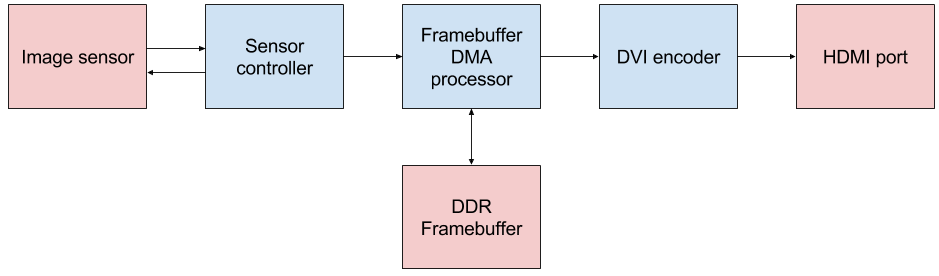
\includegraphics[width=1\textwidth]{./img/sensor_module_diagram.png}
  \caption{High-level overview of sensor module.}
  \label{fig:sensor_module_diagram}
\end{figure}

\begin{figure}
  \centering
  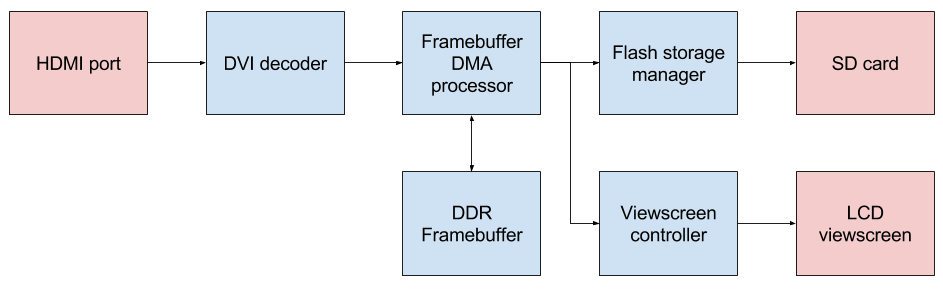
\includegraphics[width=1\textwidth]{./img/image_processor_diagram.png}
  \caption{High-level overview of the image processor inside the camera body.}
  \label{fig:image_processor_diagram}
\end{figure}

The flow of data is from left to right and starts at the OV7670 image sensor. A sensor controller block connected to the image sensor configures the internal registers and then starts capturing image data at 30 frames-per-second. Each frame captured is stored in a central framebuffer which resides in off-chip DDR3 RAM on the sensor module board where it can be accessed by a DVI encoder which is constantly working in the background and taking each from to encode it for transmission. The sensor module and image processor boards are connected using a HDMI cable. It is important to note that while a HDMI connector is present on both boards, the pins can be driven to implement whatever custom interface is desired as they are attached directly to the \gls{fpga}.

Each frame that is transmitted over the link is received and decoded by the DVI decoder on the image processor board. Decoded frames are copied into a second framebuffer, again located in off-chip DDR3 RAM. If the shutter release button is pressed then the flash storage manager takes the frame currently residing in the framebuffer and writes it to the SD card. A VGA port on the image processor board can be connected to a viewscreen LCD for real-time image display.

\section{OV7670 sensor controller}
\subsection{Overview}
To prove that the interface was suitable for image sensors a 640 x 480 OV7670 CMOS sensor was used to capture real-time image data... The Omnivision OV7670 is a small, low-cost CMOS sensor originally design for use in mobile phones which has seen popularity in the hobbyist electronics community due to its availability and ease of use. These factors, along with the wealth of documentation available contributed to its inclusion in this proof-of-concept system. As mobile phones at the time lacked the power to do image processing themselves, the OV7670 contains built-in hardware for image enhancements such as de-bayering, lens correction and noise removal, making it surprisingly complex. The OV7670 was included solely to demonstrate the effectiveness of the interface in a real camera system, thus these features are not used.

\begin{figure}
  \centering
  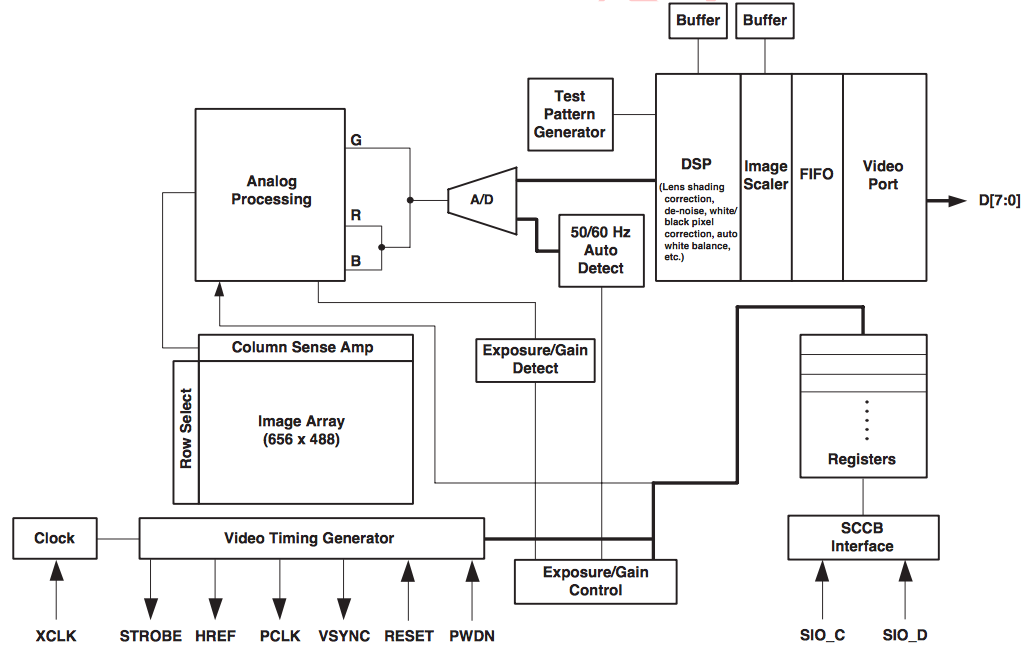
\includegraphics[width=1\textwidth]{./img/ov7670_block_diagram.png}\par
Source: Omnivision OV7670/OV7171 1.0 Specification
  \caption{Functional block diagram of Omnivision's OV7670 CMOS image sensor.}
  \label{fig:ov7670_block_diagram}
\end{figure}

Figure \ref{fig:ov7670_block_diagram} outlines the key functional blocks inside the OV7670. Light is captured by a 656 x 488 array over a specific duration of exposure. From here it is read out one row at a time into the analogue processing block which performs white-balance adjustments and amplifies the signal to increase sensitivity. From here it is digitised and fed into an image processing block for lens correction, de-noising and various other enhancements. Image scaling is also performed, before it is piped into a \gls{fifo} buffer ready for output on the 8-bit parallel video interface. The pixel size depends on the pixel format used: the RAW format only uses 8 bits and a single pixel can be output each clock cycle, while the RGB 4:2:2 and YUV 4:2:2 formats require 16 bits, thus taking two clock cycles per pixel. To construct a complete frame from the output pixels we require some additional information provided by the video timing generator in the form of vertical and horizontal synchronisation signals. The synchronisation signals in Figure \ref{fig:ov7670_timing} can be used to keep track of the starting point for each frame, and signals whether or not the pixel data on \texttt{D} can be sampled. 

\begin{figure}
  \centering
  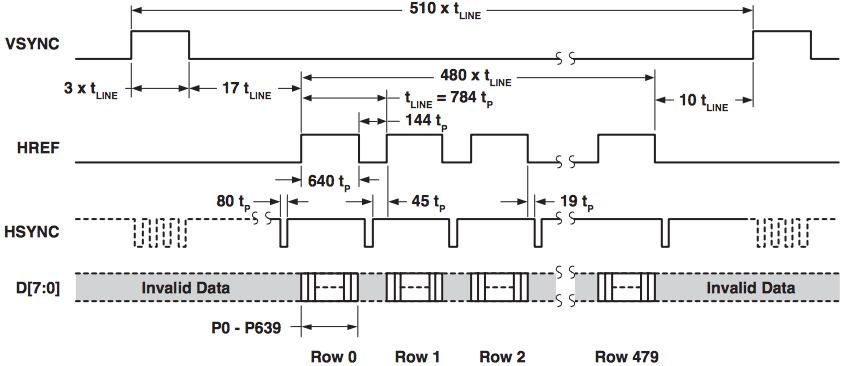
\includegraphics[width=1\textwidth]{./img/ov7670_timing.png}\par
Source: Omnivision OV7670/OV7171 1.0 Specification
  \caption{OV7670 timing diagram. The \texttt{VSYNC} signal pulses shortly before the start of each frame. \texttt{HREF} is high to indicate the data on output \texttt{D} is valid.}
  \label{fig:ov7670_timing}
\end{figure}

\subsection{\texttt{ov7670\_controller} module}
The OV7670 contains a set of internal registers to configure all aspects of its operation. In order to set the output format to 640 x 480 RAW the correct registers must be set using the \gls{sccb} protocol --- a direct clone of I\textsuperscript{2}C, renamed for licensing / IP reasons. As we are only interested in writing to specific registers there is no need to implement bidirectional I\textsuperscript{2}C communication. To drive the \gls{sccb} interface the \texttt{ov7670\_controller} module utilises I\textsuperscript{2}C code written by Mike Fields (http://hamsterworks.co.nz/mediawiki/index.php/Zedboard\_OV7670). Table \ref{table:ov7670_register_settings} lists the register settings used to configure the OV7670 for 640 x 480 RAW output at 30 \gls{fps}. On powerup, the \texttt{ov7670\_controller} module performs the following actions for each register it configures:

\begin{enumerate}
    \item Pull \texttt{SDA} low to signal master is about to send
    \item Send 8-bit address frame with value 0x42
        \begin{itemize}
            \item \texttt{Bits 7--1}: OV7670 I\textsuperscript{2}C slave address \texttt{0x21}
            \item \texttt{Bit 0}    : \texttt{R/W = 0} to write to register) 
        \end{itemize}
    \item Pause to allow OV7670 to acknowledge address frame
    \item Send 8-bit data frame with address of configuration register
    \item Pause to allow OV7670 to acknowledge data frame
    \item Send a second data frame with value to write to configuration register
    \item Pause to allow OV7670 to acknowledge data frame
\end{enumerate}

The \texttt{ov7670\_controller} module contains a 'dumb' I\textsuperscript{2}C controller --- it ignores all responses from the slave and stops as soon as it has finished configuring the OV7670 registers. For the sake of simplicity, the register configuration can be re-triggered by asserting the reset signal. Not implementing intelligence to deal with frame retransmits due to errors simplifies the design significantly, while still allowing the user to manually re-trigger register configuration if anything does go wrong. Once the configuration has been written the \texttt{ov7670\_controller} module asserts the \texttt{start\_capture} signal to notify the \texttt{ov7670\_capture} module that the OV7670 is initialised and properly configured.

\begin{table}
    \begin{tabular}{llll}
    Register            & Address   & Value     & Description                       \\
    COM7                & 0x12      & 0x80      & Reset all registers to defaults   \\
    CLKRC               & 0x11      & 0x01      & Input clock prescaler divide-by-four, disable PCLK doubling (PCLK will be \(f_internal / 2\)) \\
    DBLV                & 0x6B      & 0x7A      & Input clock PLL x4                \\
    COM7                & 0x12      & 0x01      & Output format 640 x 480 Bayer RAW \\
    COM3                & 0x0C      & 0x00      & Disable output scaling            \\
    COM14               & 0x3E      & 0x00      & No PCLK scaling                   \\
    SCALING\_XSC         & 0x70      & 0x3A      & Magical horizontal scale factor   \\
    SCAKING\_YSC         & 0x71      & 0x35      & Magical vertical scale factor     \\
    SCALING\_DCWCTR      & 0x72      & 0x11      & Downsample by 2           \\
    SCALING\_PCLK\_DIV    & 0x73      & 0xF0      & No PCLK scaling           \\
    SCALING\_PCLK\_DELAY  & 0xA2      & 0x02      & Scaling output delay 2    \\
    \end{tabular}
    \caption{(Based on values in OV7670 datasheet and implementation guide)}
    \label{table:ov7670_register_settings}
\end{table}

\subsection{\texttt{ov7670\_capture} module}
Given that the purpose of a standardised image sensor interface is to provide video data in a format which can be paired with any image sensor device, it stands to reason that the data must be converted to a different format at some point. The task of the \texttt{ov7670\_capture} module is to capture pixels from the OV7670's parallel video interface and pass them on to the \texttt{i\_buf\_controller} module detailed in Section \ref{sec:framebuffer_dma} for storage in the framebuffer where they are processed by the DVI encoder. Originally the \texttt{ov7670\_capture} module had direct control over the memory, however this functionality was moved to the \texttt{i\_buf\_controller} module, reducing the \texttt{ov7670\_capture} to a passthrough or level conversion device.

To transfer frames between different blocks inside the \gls{fpga}, uses the standard VESA video interface: a pixel clock to signal when a new pixel is available, parallel data for pixels, horizontal sync for signalling end-of-line, vertical sync for signalling end-of-frame, and additionally a data valid signal which marks exactly when the active video period begins---greatly simplifying the design. Without this signal a timing recovery block would be needed to measure the frequency of \texttt{vsync} and \texttt{hsync} pulses to determine the resolution of the video and thus where the active video period begins and ends.

The OV7670's video interface is very similar, however some signals are lacking and others function differently as summarised in Table \ref{table:ov7670_video_interface}. 

\begin{table}
  \begin{tabular}{lll}
  OV7670 signal   & VESA equivalent & Description                                           \\
  d[7:0]          & d[7:0]          & Pixel data remains the same                           \\
  vsync           & vsync           & OV7670 vsync is active-high, VESA vsync is active-low \\
  href            & vde             & href is active-low, vde is active-high                \\
  N/A             & hsync           & OV7670 lacks a href signal
  \end{tabular}
  \caption{The OV7670 video interface is very similar to the VESA interface, however minor signal conversions are required.}
  \label{table:ov7670_video_interface}
\end{table}
\section{Framebuffer DMA processor}
\label{sec:framebuffer_dma}

A framebuffer is a portion of memory which holds the current frame, allowing the hardware blocks either side to act in complete isolation. Both sides of the link use framebuffers, though their purpose differs. On the receiver side the framebuffer stores each frame before it is written to flash storage. Firmware inside the Zynq \gls{ps} \marginpar{Explain the Zynq PS} can draw to the frame in real-time, adding helpful indicators such as the currently connected sensor module and gridlines to aid the photographer's composition process. On the transmitter side the framebuffer serves a different purpose. A critical flaw in the design of the \gls{dvi} receiver causes the link to break if the incoming pixel clock is less than \SI{40}{\mega\hertz} --- a potential issue because the OV7670's pixel clock is only \SI{12}{\mega\hertz}. To mitigate this, the transmitter sends out duplicate frames, thus bringing the pixel clock up into the region required for correct operation.

The space required to store frames is a direct function of the image resolution. As the OV7670 outputs frames in 640 x 480 resolution, a \SI{307.2}{\kilo\byte} framebuffer is required. While \glspl{fpga} usually contain a small amount of internal block RAM, there is insufficient space for storing an entire frame. Though its access is significantly more complicated, the Zynq-7000 includes a hard DDR controller which can be utilised to store the frames in external DDR3 memory instead --- the Zybo development board contains \SI{512}{\mega\byte} of RAM, which is more than sufficient for storing a single frame.

\marginpar{Diagram of internal Zynq arch - access to DDR}

\subsection{AXI}
Due to the internal architecture of the Zynq-7000, external RAM is only accessible from the \gls{ps}, thus incoming frames which are processed by the \gls{pl} must be fed into the \gls{ps} before they can be stored in the RAM. Fortunately the \gls{pl} and \gls{ps} are able to exchange data using the \gls{axi} interface, which was designed to provide a single interconnect for IP across all domains. While there are several different variants of \gls{axi} (a comparison of which is found in Table \ref{table:axi_comparison}), they all operate in fundamentally the same way. \gls{axi} is used to connect a master device to a slave device using one or more channels which are used to carry out transactions. A standard AXI4 connection will consist of five channels:
\begin{itemize}
  \item Read Address Channel
  \item Write Address Channel
  \item Read Data Channel
  \item Write Data Channel
  \item Write Response Channel
\end{itemize}
(http://www.xilinx.com/support/documentation/ip_documentation/axi_ref_guide/latest/ug1037-vivado-axi-reference-guide.pdf)

\begin{table}[]
\centering
\caption{Comparison of AXI interfaces. Adapted from (http://www.xilinx.com/support/documentation/ip_documentation/axi_ref_guide/latest/ug1037-vivado-axi-reference-guide.pdf).}
\label{table:axi_comparison}
\begin{tabular}{llll}
              & AXI4                               & AXI4-Lite                      & AXI4-Stream                \\
Dedicated for & High-performance and memory-mapped & Register-style interfaces      & Non-address based IP       \\
Burst         & Up to 256                          & 1                              & Unlimited                  \\
Data width    & 32 - 1024 bits                     & 32 / 64 bits                   & Anything                   \\
Applications  & Embedded, memory                   & Small footprint logic, control & DSP, video, communications
\end{tabular}
\end{table}

As separate channels are used for reading and writing, device communication is fully bi-directional. In addition to the address and data signals, extra signals are provided for control and synchronisation to ensure that a device can only begin a transaction when the other device is ready. Figure \ref{fig:axi_architecture} illustrates a typical AXI4 interface. 

\begin{figure}
\centering
\begin{subfigure}{.5\textwidth}
  \centering
  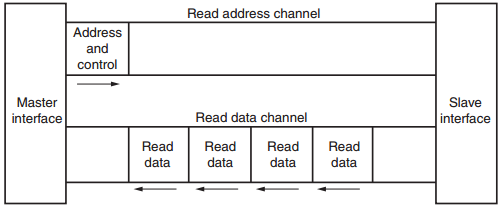
\includegraphics[width=.4\linewidth]{./img/axi_read.png}
  \caption{Read Channel}
\end{subfigure}%
\begin{subfigure}{.5\textwidth}
  \centering
  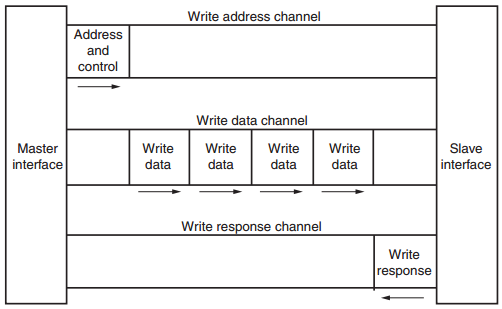
\includegraphics[width=.4\linewidth]{./img/axi_write.png}
  \caption{Write Channel}
\end{subfigure}
\caption{Architecture of AXI4 Read and Write Channels. (http://www.xilinx.com/support/documentation/ip_documentation/axi_ref_guide/latest/ug1037-vivado-axi-reference-guide.pdf)}
\label{fig:axi_architecture}
\end{figure}

All hardware inside the Zynq can be addressed from the \gls{ps} provided it has been connected via \gls{axi}. AXI requires all devices to be assigned an address which complies with the address map in Table \ref{table:zynq_address_map}. For example, the \gls{axi} master port \texttt{M\_AXI\_GP0} on the \gls{ps} has the address range \texttt{0x4000_0000} to \texttt{0x7FFF_FFFF}. Any \gls{axi} slave devices in the \gls{pl} assigned an address in this range can be accessed from the \gls{ps}. Conversely, any \gls{axi} master devices in the \gls{pl} connected to the \gls{ps} slave port \texttt{S\_AXI\_HP0} can access most of the DDR address range.

\begin{table}[]
\centering
\caption{Zynq-7000 system-level address map. (http://www.xilinx.com/support/documentation/user_guides/ug585-Zynq-7000-TRM.pdf)}
\label{table:zynq_address_map}
\begin{tabular}{lllll}
Address range                             & CPUs and ACP & AXI\_HP & Other bus masters & Notes                                                 \\
\multirow{4}{*}{0000\_0000 to 0003\_FFFF} & OCM          & OCM     & OCM               & Address not filtered by SCU and OCM is mapped low     \\
                                          & DDR          & OCM     & OCM               & Address filtered by SCU and OCM is mapped low         \\
                                          & DDR          &         &                   & Address filtered by SCU and OCM is not mapped low     \\
                                          &              &         &                   & Address not filtered by SCU and OCM is not mapped low \\
\multirow{2}{*}{0004\_0000 to 0007\_FFFF} & DDR          &         &                   & Address filtered by SCU                               \\
                                          &              &         &                   & Address not filtered by SCU                           \\
\multirow{2}{*}{0008\_0000 to 000F\_FFFF} & DDR          & DDR     & DDR               & Address filtered by SCU                               \\
                                          &              & DDR     & DDR               & Address not filtered by SCU                           \\
0010\_0000 to 3FFF\_FFFF                  & DDR          & DDR     & DDR               & Accessible to all interconnect masters                \\
4000\_0000 to 7FFF\_FFFF                  & PL           &         & PL                & General Purpose Port \#0 to the PL, M\_AXI\_GP0       \\
8000\_0000 to BFFF\_FFFF                  & PL           &         & PL                & General Purpose Port \#1 to the PL, M\_AXI\_GP1       \\
E000\_0000 to E02F\_FFFF                  & IOP          &         & IOP               & I/O Peripheral registers                              \\
E100\_0000 to E5FF\_FFFF                  & SMC          &         & SMC               & SMC Memories                                          \\
F800\_0000 to F800\_0BFF                  & SLCR         &         & SLCR              & SLCR registers                                        \\
F800\_1000 to F880\_FFFF                  & PS           &         & PS                & PS System registers                                   \\
F890\_0000 to F8F0\_2FFF                  & CPU          &         &                   & CPU Private registers                                 \\
FC00\_0000 to FDFF\_FFFF                  & Quad-SPI     &         & Quad-SPI          & Quad-SPI linear address for linear mode               \\
\multirow{2}{*}{FFFC\_0000 to FFFF\_FFFF} & OCM          & OCM     & OCM               & OCM is mapped high                                    \\
                                          &              &         &                   & OCM is not mapped high                               
\end{tabular}
\end{table}

\marginpar{Include address map of actual design}

\subsection{Linebuffers}
Due to the high complexity of the DDR controller, memory operations are not instantaneous and have non-deterministic latencies, thus an additional buffer must be placed between the incoming frames from the \texttt{ov7670\_capture} block and framebuffer, and a second between the framebuffer and the \texttt{rgb2dvi} module.

Each line of the input frame is written into a \SI{2048}{\kilo\bit} linebuffer pixel-by-pixel. 

During the blanking period an interrupt on the \gls{ps} is triggered 

\subsection{\texttt{i\_buf\_controller} module}

The \texttt{i_buf_controller} module is a simple shim which writes each line of the video into the linebuffer and triggers interrupts on the \gls{ps} to initiate a \gls{dma} transfer into the DDR framebuffer. Upon detecting the \texttt{vde} signal going high, the input buffer controller starts writing each incoming pixel into the linebuffer. The block RAM can either be configured in standalone mode or for use with an AXI BRAM Controller instance. The block RAM has its own address space (starting at \texttt{0x0000} up to however large the block RAM is), and so an AXI BRAM Controller instance is placed between the block RAM and input AXI CDMA instance (\texttt{i\_axi\_cdma}) to translate between the two address spaces.

As the block RAM is operating in BRAM Controller mode the following Block Memory Generator configuration is used:
\begin{itemize}
  \item 32-bit data width
  \item 2048-bit data depth
  \item 32-bit address width
  \item Byte addressing

\subsection{AXI CDMA and buffer control firmware}


\marginpar{Diagram of OV7670 -> framebuffer -> DVI isolation, and DVI -> framebuffer -> SD / screen}
\section{DVI encoder}

\marginpar{Include formula for exact throughput, and pixel clocks used for OV7670}

The \gls{dvi} encoder and decoder presented here are based heavily upon a reference design provided by Digilent's IP library for the Zybo development board. Rather than reinvent the wheel, this project opts to use these cores as a base and extend them for use with image sensors. All third-party code has been attributed, as per the BSD-license which the IP is released under. Custom additions have been marked.

\subsection{\texttt{rgb2dvi} module overview}
\begin{figure}
  \centering
  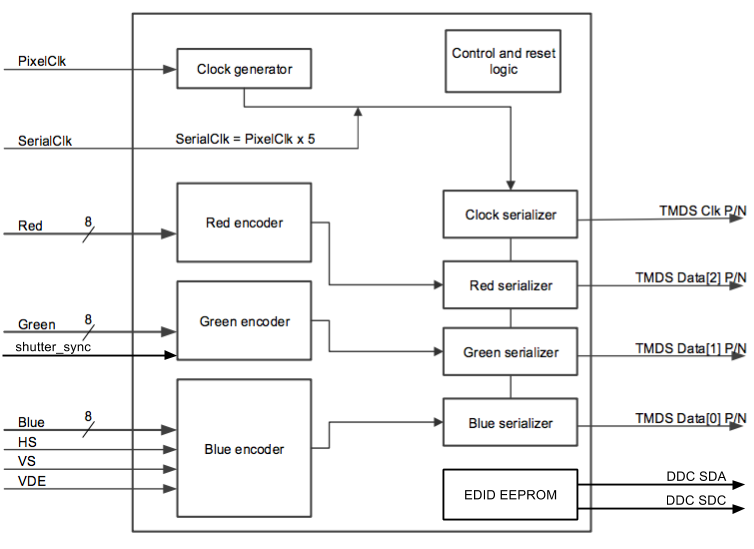
\includegraphics[width=1\textwidth]{./img/rgb2dvi.png}
  \caption{Block diagram of the DVI encoder \cite{rgb2dvi}.}
  \label{fig:rgb2dvi}
\end{figure}

The \gls{dvi} encoder takes a 24-bit wide pixel data bus as the main input, splitting off into three 8-bit channels for Red, Green and Blue. As the application requires a RAW pixel format instead of RGB we must deviate from the \gls{dvi} specification slightly by combining all channels into one large input, however internally they are still treated separately. Only a single channel (Blue) is used for data in the proof-of-concept as the OV7670 only has an 8-bit \gls{adc}, however the Green channel is also used to transmit the control signals related to flash and shutter synchronisation. Combining all channels gives a maximum pixel depth of 24-bits --- the image sensor on a professional \gls{dslr} will typical have a 12--14-bit \gls{adc}, so 24-bits is more than sufficient. Alongside the pixel bus are the regular video timing and synchronisation signals used elsewhere in the design. In addition to these timing signals, a \texttt{shutter\_sync} signal has been added which fires just before each new frame so that the receiver side can sequence a mechanical shutter or flash if present. Much like the video timing signals, the shutter synchronisation signal is sent via the control bits on the Green channel.

Internally the \gls{dvi} encoder instantiates three identical \texttt{TMDS\_encoder} blocks and assigns each one to a channel. Immediately after each \gls{tmds} encoder is an \texttt{OutputSERDES} block which is what actually drives the \gls{tmds}-encoded data across the interface. Listing \ref{lst:encoder_instances} shows how the \texttt{generate} statement is used to create three identical instances of the \texttt{TMDS\_encoder} and \texttt{OutputSERDES} blocks.

\begin{lstlisting}[caption={Instantiatiating a TMDS encoder and serialiser for each channel.}, label={lst:encoder_instances}, language=VHDL]
DataEncoders: for i in 0 to 2 generate
   DataEncoder: entity work.TMDS_Encoder
      port map (
         PixelClk => PixelClk,
         SerialClk => SerialClk,
         pDataOutRaw => pDataOutRaw(i),
         aRst => pRstLck,
         pDataOut => pDataOut(i),
         pC0 => pC0(i),
         pC1 => pC1(i),
         pVde => pVde(i)
      );
   DataSerializer: entity work.OutputSERDES
      generic map (
         kParallelWidth => 10) -- TMDS uses 1:10 serialization
      port map(
         PixelClk => PixelClkIO,
         SerialClk => SerialClkIO,
         sDataOut_p => TMDS_Data_p(i),
         sDataOut_n => TMDS_Data_n(i),
         --Encoded parallel data (raw)
         pDataOut => pDataOutRaw(i),
         aRst => pRstLck);      
end generate DataEncoders;
\end{lstlisting} 

\subsection{TMDS encoding}
As covered in the section on the \gls{dvi} interface, \gls{tmds} encoding is utilised in order to minimise data transitions (and thus \gls{emi}) and provide a \gls{dc} balance, which it does by mapping each 8-bit input to a unique 10-bit \gls{tmds} character.

The flowchart in Figure \ref{fig:tmds_encoding_algorithm} outlines the algorithm used for \gls{tmds} encoding. The notation is as follows \cite{dvi_spec}:
\begin{itemize}
    \item \texttt{D C0 C1 DE}: The input set of the encoder. D is an 8-bit pixel data value, C0 and C1 are the two control bits and DE indicates whether the data is valid.
    \item \texttt{cnt}: This register indicates the disparity of the data stream. A value \texttt{1} in the bit stream will increment the counter, and a \texttt{0} will decrement it. \texttt{cnt(t-1)} refers to the register value for the previous bit of data, and \texttt{cnt(t)} is the register value for the current bit of input data.
    \item \texttt{q\_out}: The \gls{tmds}-encoded output value.
    \item N\textsubscript{1}\{x\}: Number of \texttt{1}s in \texttt{x}.
    \item N\textsubscript{0}\{x\}: Number of \texttt{0}s in \texttt{x}.
\end{itemize}

The encoding algorithm can be split into three discrete pipeline stages:
\begin{enumerate}
    \item Transition minimisation
    \item DC balancing
    \item Output registering
\end{enumerate}

\begin{lstlisting}[caption={TMDS encoder transition minimisation stage.}, label={lst:encoder_stage_1}, language=VHDL]
-- Pipeline stage 1, minimise transitions
----------------------------------------------------------------------------------
Stage1: process(PixelClk)
begin
    if Rising_Edge(PixelClk) then
        pVde_1 <= pVde;

        n1d_1 <= sum_bits(pDataOut(7 downto 0));
        pDataOut_1 <= pDataOut; --insert data into the pipeline;
        pC0_1 <= pC0; --insert control into the pipeline;
        pC1_1 <= pC1;
    end if;
end process Stage1;

----------------------------------------------------------------------------------
-- Choose one of the two encoding options based on n1d_1
----------------------------------------------------------------------------------
q_m_xor_1(0) <= pDataOut_1(0);
encode1: for i in 1 to 7 generate
    q_m_xor_1(i) <= q_m_xor_1(i-1) xor pDataOut_1(i);
end generate encode1;
q_m_xor_1(8) <= '1';

q_m_xnor_1(0) <= pDataOut_1(0);
encode2: for i in 1 to 7 generate
    q_m_xnor_1(i) <= q_m_xnor_1(i-1) xnor pDataOut_1(i);
end generate encode2;
q_m_xnor_1(8) <= '0';

q_m_1 <= q_m_xnor_1 when n1d_1 > 4 or (n1d_1 = 4 and pDataOut_1(0) = '0') else
         q_m_xor_1;

n1q_m_1 <= sum_bits(q_m_1(7 downto 0));
\end{lstlisting}

The first stage, in Listing \ref{lst:encoder_stage_1} aims to minimise the number of transitions in the data by XORing with previous inputs. After counting the ones and zeros in the input bits, the intermediate \texttt{q\_m} bits are set by XORing them with the current data bits. An additional 9\textsuperscript{th} intermediate bit is set to either \texttt{1} if the input data contains less than four ones, or \texttt{0} otherwise.

\begin{lstlisting}[caption={TMDS encoder DC balancing stage.}, label={lst:encoder_stage_2}, language=VHDL]
----------------------------------------------------------------------------------
-- Pipeline stage 2, balance DC
----------------------------------------------------------------------------------
Stage2: process(PixelClk)
begin
    if Rising_Edge(PixelClk) then
        n1q_m_2 <= n1q_m_1;
        n0q_m_2 <= 8 - n1q_m_1;
        q_m_2 <= q_m_1;
        pC0_2 <= pC0_1;
        pC1_2 <= pC1_1;
        pVde_2 <= pVde_1;
    end if;
end process Stage2;

cond_balanced_2 <=   '1' when cnt_t_3 = 0 or n1q_m_2 = 4 else -- DC balanced output
                           '0';
cond_not_balanced_2 <=  '1' when (cnt_t_3 > 0 and n1q_m_2 > 4) or -- too many 1's
                                     (cnt_t_3 < 0 and n1q_m_2 < 4) else -- too many 0's
                        '0';

control_token_2 <=  kCtlTkn0 when pC1_2 = '0' and pC0_2 = '0' else
                     kCtlTkn1 when pC1_2 = '0' and pC0_2 = '1' else
                     kCtlTkn2 when pC1_2 = '1' and pC0_2 = '0' else
                     kCtlTkn3;
                            
q_out_2 <=  control_token_2                                             when pVde_2 = '0' else  --control period
               not q_m_2(8) & q_m_2(8) & not q_m_2(7 downto 0)    when cond_balanced_2 = '1' and q_m_2(8) = '0' else
               not q_m_2(8) & q_m_2(8) & q_m_2(7 downto 0)        when cond_balanced_2 = '1' and q_m_2(8) = '1' else
               '1' & q_m_2(8) & not q_m_2(7 downto 0)             when cond_not_balanced_2 = '1' else
               '0' & q_m_2(8) & q_m_2(7 downto 0);  --DC balanced

dc_bias_2 <= signed('0' & n0q_m_2) - signed('0' & n1q_m_2);

cnt_t_2 <=  to_signed(0, cnt_t_2'length)                                   when pVde_2 = '0' else   --control period
               cnt_t_3 + dc_bias_2                                            when cond_balanced_2 = '1' and q_m_2(8) = '0' else
               cnt_t_3 - dc_bias_2                                            when cond_balanced_2 = '1' and q_m_2(8) = '1' else
               cnt_t_3 + signed('0' & q_m_2(8 downto 8) & '0') + dc_bias_2     when cond_not_balanced_2 = '1' else
               cnt_t_3 - signed('0' & not q_m_2(8 downto 8) & '0') - dc_bias_2;
\end{lstlisting}

A second stage, shown in Listing \ref{lst:encoder_stage_2}, aims to balance the overall \gls{dc} offset of the bit stream. If the \texttt{VDE} signal is low then this step is bypassed altogether as this indicates that we are now in the blanking period and should only be sending control data. During the blanking period the input pixel data is completely ignored, instead the control signals are encoded directly using a \gls{lut} to produce one of four unique 10-bit control tokens, depending on the relevant combination of control inputs \texttt{C0} and \texttt{C1}. These control tokens have been specially picked to be easy to detect at the receiver in order to aid phase alignment. If we are in the active video period then the process is significantly more complex and involves counting the number of ones and zeros in the intermediate values to determine what value to clock into the output registers.

The stage of the pipeline clocks the intermediate values into an output register, \texttt{q\_out}, where they are then passed on to the serialiser.

\subsection{Serialisation}

Originally written in VHDL, the serialiser code was re-written in Verilog as part of this project. To obtain the highest data rates that the \gls{fpga} is capable of it is necessary to use Xilinx's OSERDESE2 primitives, which take the 10-bit output characters from the \gls{tmds} encoder and two clocks (one parallel clock and a serial higher serial clock) and then serialises them into a single-bit high-speed output stream. The OSERDESE2 primitive only has an 8-bit input which is too narrow for the 10-bit \gls{tmds} output. To achieve the 10:1 serialisation ratio required, two OSERDESE2 primitives operating in \gls{ddr} mode must be chained together as in Figure \ref{fig:10_1_serdes}. The inputs to the OSERDESE2 primitives are swapped as \gls{dvi} sends the least significant bit first, whereas the OSERDESE2 primitives send \texttt{D1} first.

When configured as a cascaded 10:1 \gls{ddr} topology the OSERDESE2 primitive has an output latency of 5 clock cycles \cite{xilinx:ug471}. To ensure that the \gls{tmds} clock channel is correctly aligned with the data channels it is also run through a serialiser, adding 5 cycles of latency to bring it back in line with the rest of the data.

\begin{figure}
  \centering
  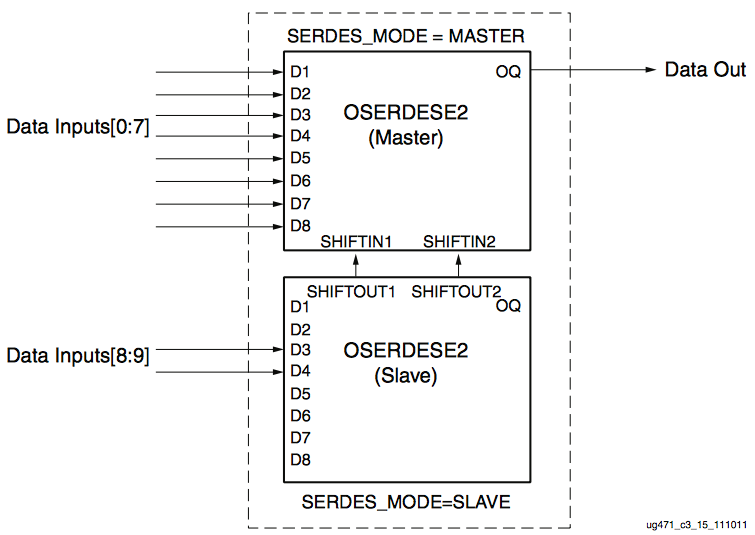
\includegraphics[width=1\textwidth]{./img/10_1_serdes.png}
  \caption{10:1 serialisation is achieved by chaining two OSERDES2 primitives in DDR mode \cite{xilinx:ug471}.}
  \label{fig:10_1_serdes}
\end{figure}

\subsection{DDC channel}

While the video sink is usually the I\textsuperscript{2}C master of the \gls{ddc} channel, the proof-of-concept design instead assigns the video source (image sensor) as the master so that it may advertise its capabilities to the camera body. The \gls{ddc} code is part of Digilent's IP library and uses internal memory resources to store a 128-byte \gls{edid} and presents itself as an I\textsuperscript{2}C-attached \gls{eeprom}. The \gls{edid} implementation is detailed in Section \ref{sec:edid}.

\subsection{Clocking}
Three clocks --- all of which are generated externally --- are required for the \gls{dvi} encoder to function correctly:
\begin{itemize}
    \item \texttt{PixelClk}: One tick for every pixel
    \item \texttt{SerialClk}: Feeds the OSERDESE2 primitives, must be 5x the frequency of the PixelClk due to the 10:1 serialisation ratio and use of \gls{ddr} mode
    \item \texttt{RefClk}: Drives the I\textsuperscript{2}C-attached \gls{eeprom} for the \gls{edid}
\end{itemize}

The route between the serial clock and the OSERDESE2 primitives is without doubt the most critical part of the entire design as it limits the maximum throughput. To ensure that the tools have the best possible chance of meeting the throughput requirements the serial clock is constrained to be five times the pixel clock frequency, as in Listing \ref{lst:timing_constraints}

\begin{lstlisting}[caption={Serial clock timing constraints}, label={lst:timing_constraints}, language=tcl]
### Clock constraints ###
create_generated_clock -source [get_ports PixelClk] -multiply_by 5 [get_ports SerialClk]
\end{lstlisting}

\subsection{Performance}
Performance is ultimately limited by the Zynq-700's F\textsubscript{MAX\_BUFIO} figure, specified as \SI{710}{\mega\hertz}\cite{xilinx:ds187}. F\textsubscript{MAX\_BUFIO} is the maximum switching rate of the input / output clock tree, meaning that any IO buffers cannot operate any higher than \SI{710}{\mega\hertz}. The highest resolution is thus the one which corresponds to a pixel clock of \SI{142}{\mega\hertz}, which is just shy of the \SI{148.5}{\mega\hertz} pixel clock required for 1080p. Because silicon vendors are normally conservative with their specifications, it turns out that even though the timing constraints are not met during place and route, the Zybo development board used for the proof-of-concept can actually operate outside of its specification, and can just about manage to transmit and receive 1080p video.
\section{DVI decoder}

\subsection{\texttt{dvi2rgb} module overview}
\begin{figure}
  \centering
  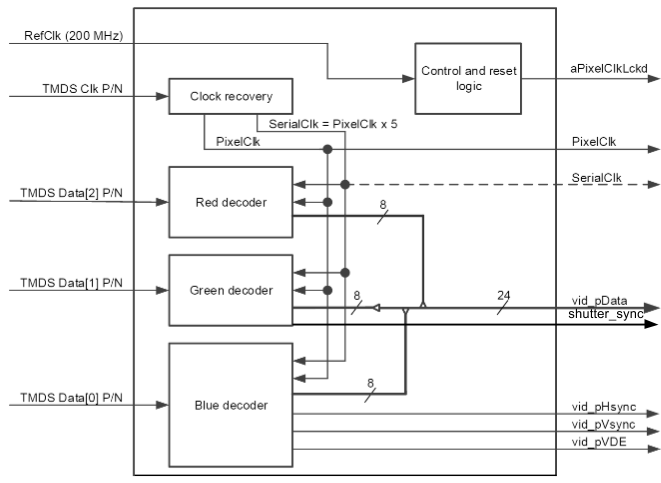
\includegraphics[width=0.8\textwidth]{./img/dvi2rgb.png}\par
  \caption{Block diagram of the DVI decoder \cite{dvi2rgb}.}
  \label{fig:dvi2rgb}
\end{figure}

The DVI decoder is connected via a \gls{hdmi} cable to the output of the DVI encoder on the sensor module board. It is important to note that the \gls{hdmi} port is connected directly to the \gls{fpga} and can be used to transmit anything provided the \gls{fpga} is configured correctly. The \gls{hdmi} ports have been carefully routed to carry four high-speed differential signals --- their controlled impedance makes them ideally suited to cope with the required bandwidth. As with the encoder, each channel is independent and so three identical decoders are instantiated, the output of which is concatenated to produce a 24-bit pixel bus accompanied by the standard video timing and synchronisation signals which are derived from the control data bits. In this proof-of-concept system the 8-bit pixel values from the OV7670 are tapped from the Blue channel on the receiver, a single control bit for the shutter synchronisation signal is tapped from the Green channel, and the Red channel remains unused.

\section{Clock recovery}
As the system is source-synchronous, the \gls{dvi} clock channel is used to drive the \gls{dvi} decoder logic on the receiver. The clock channel cannot be used directly, rather it contains a character-rate reference signal which is fed into a \gls{pll} to generate the pixel clock and serial clocks needed for the decoder logic to function. To generate these clocks an MMCME2\_ADV primitive, providing clock management functionality, is instantiated inside the \gls{dvi} decoder. Figure \ref{fig:clock_recovery} illustrates how the differential \gls{tmds} clock is fed into a differential input global clock buffer (\texttt{IBUFGDS}) connected to the input of the \gls{mmcm} primitive. The \gls{mmcm} contains a \gls{pll} clock multiplier which locks on to the reference clock and generates an output clock with a frequency five times higher. The output clock from the \gls{mmcm} is split and fed into two buffers. The first, a \texttt{BUFIO} primitive, provides the serial clock for the \texttt{ISERDESE2} primitives in the deserialisation logic. The second buffer is a \texttt{BUFR} primitive which has a frequency divider on it, which is used to divide the 5x serial clock back down and thus is how the pixel clock is generated. 

\begin{figure}
  \centering
  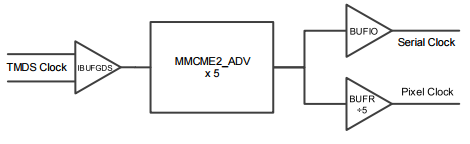
\includegraphics[width=0.8\textwidth]{./img/clock_recovery.png}
  \caption{Clock recovery overview \cite{dvi2rgb}.}
  \label{fig:clock_recovery}
\end{figure}

Inside the \gls{pll} a \gls{vco} is used is to generate an internal clock which can be varied by the feedback loop until it is locked to the reference clock \texttt{TMDS\_Clk}. The \gls{vco} operates at a frequency of \(FVCO = FIN * MULT_F\), meaning for an input \texttt{PixelClk} of \SI{12}{\mega\hertz} (as is the case with the OV7670), the \gls{vco} would oscillate at \SI{60}{\mega\hertz} due to the x5 multiplier. Unfortunately the \gls{vco} has a limited operating range between \SI{600}{\mega\hertz} and \SI{1200}{\mega\hertz}, to work with a \SI{12}{\mega\hertz} reference clock, the multiplier would need to be set to 50 to bring it up into the correct operating range, and then the output clock would need dividing by 10 to restore the 1:5 input / output ratio \cite{xilinx:ds187}.

Using the simple Python script in Listing \ref{lst:pll_calc} to naively search through the entire parameter space, no single set of PLL parameters will satisfy the full range of input frequencies while operating within the \gls{vco} limits. This means that the input frequency must be known prior to synthesis so the correct \gls{pll} parameters can be set. However, it is not uncommon for manufacturers to be conservative with their limits, and it happens that the \gls{vco} can operate far below the specified limits --- all of the tests performed were done with the gls{pll} parameters set for a \texttt{PixelClk} of \SI{148.5}{\mega\hertz}, despite the actual input being \SI{50}{\mega\hertz}. 

\begin{lstlisting}[caption={PLL parameter calculator script.}, label={lst:pll_calc}, language=Python]
"""A small script to calculate PLL parameters for target clocks.
This is easily the least efficient way to do it, but the search space
is pretty small so it's easier to just brute-force it. A parametric
solver would be better....

"""

CLK_IN1 = [25.175, 148.5]
TARGET = 5
TOLERANCE = 1   # +/- 1 Hz

DIVCLK_DIVIDE = xrange(1, 107)
CLKFBOUT_MULT = xrange(2, 65)
CLKOUT0_DIV = xrange(1, 129)
FVCOMIN = 600
FVCOMAX = 1200

print("{:<13} {:<13} {:<11}".format('DIVCLK_DIVIDE', 'CLKFBOUT_MULT', 'CLKOUT0_DIV'))

for divclk in DIVCLK_DIVIDE:
    for mult in CLKFBOUT_MULT:
        for div in CLKOUT0_DIV:
            for clk_in in CLK_IN1:
                fvco = clk_in * mult / divclk
                fout = fvco / div
                if fvco < FVCOMIN or fvco > FVCOMAX \
                  or fout < clk_in * TARGET - TOLERANCE or fout > clk_in * TARGET + TOLERANCE:
                    solution_found = False
                    break

                solution_found = True
            
            if solution_found: 
                print("{:<13} {:<13} {:<11}".format(divclk, mult, div))
\end{lstlisting}

\section{Deserialisation}

Much like the \texttt{rgb2dvi} module, deserialisation is done by chaining together two \texttt{ISERDESE2} primitives in a cascaded 1:10 DDR topology. Unlike the transmitter, the receiver requires an additional synchronisation step to re-align the three channels with the clock channel, as they may be out-of-phase by the time they reach the receiver. To do this a 32-tap delay line \texttt{IDELAYE2} primitive is inserted in front of each \texttt{ISERDESE2} primitives. Because transistors take a finite period of time to drive the line from low to high (\textit{rise-time}) or high to low (\textit{fall-time}), it is crucial that the signal is sampled at the correct time to avoid sampling the transition point. Figure \ref{fig:eye_diagram} shows how an eye opening forms when successive signals are repeatedly overlaid to form an eye diagram. As jitter increases, the lines become thicker and the signal is stable for less time. The basic premise is to increment the delay until we find the eye opening, which provides the best place to sample the signal. The \gls{tmds} encoder sends a large string of successive control tokens during the blanking period. As the value of the control tokens is fixed, we can keep adjusting the delay increments until we sample a value which matches the 10-bit control token we expect during the blanking period. Each tap only adds a \SI{78}{\pico\second} delay, which is only enough to shift between a bit or two. To shift between entire characters (10-bits) in order to find the character boundaries requires a much greater delay, which is done using the \textit{bitslip} control inside the \texttt{ISERDESE2} primitive. The \texttt{PhaseAlign} and \texttt{ChannelBond} modules control a state machine which sequences the delay increments to ensure all three channels are aligned at the start of each blanking period.

A critical issue occurs when the input \texttt{PixelClk} frequency is below \SI{40}{\mega\hertz}, which corresponds to the maximum \SI{78}{\pico\second} delay of the delay line. With the \SI{12}{\mega\hertz} pixel clock from the OV7670, the clock period is so long that it is possible to exhaust all of the delay taps without finding stable zone inside the eye. To rectify this, the incoming pixel clock must be boosted to above \SI{40}{\mega\hertz} by injecting artificial duplicate frames at the transmitter in order to allow the eye opening to be found correctly.

\begin{figure}
  \centering
  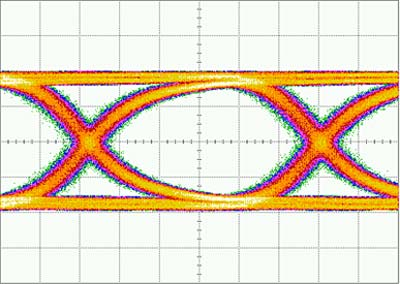
\includegraphics[width=0.5\textwidth]{./img/eye_diagram.jpg}
  \caption{\gls{serdes} eye diagram \cite{eye_diagram}.}
  \label{fig:eye_diagram}
\end{figure}

\section{TMDS decoding}

The decoding phase is far simpler than the encoding phase. A lookup table is used to see if the character matches any of the four known control tokens, and if so, sets the output accordingly. If the character is encoded data, the decoder XORs or XNORs each of the bits together to form the output.

\begin{lstlisting}[caption={TMDS decoding logic.}, label={lst:tmds_decode}, language=VHDL]
case (pDataInBnd) is
  --Control tokens decode straight to C0, C1 values
  when kCtlTkn0 =>
     pC0 <= '0';
     pC1 <= '0';
     pVde <= '0';
  when kCtlTkn1 =>
     pC0 <= '1';
     pC1 <= '0';
     pVde <= '0';               
  when kCtlTkn2 =>
     pC0 <= '0';
     pC1 <= '1';
     pVde <= '0';
  when kCtlTkn3 =>
     pC0 <= '1';
     pC1 <= '1';
     pVde <= '0';
  --If not control token, it's encoded data
  when others =>
     pVde <= '1'; 
     pDataIn(0) <= pDataIn8b(0);
     for iBit in 1 to 7 loop
        if (pDataInBnd(8) = '1') then
           pDataIn(iBit) <= pDataIn8b(iBit) xor pDataIn8b(iBit-1);
        else
           pDataIn(iBit) <= pDataIn8b(iBit) xnor pDataIn8b(iBit-1);
        end if;
     end loop;                           
end case;
\end{lstlisting}

\section{EDID subsystem}

As large parts of the system are highly-dependent on the format of the incoming video data, sensor modules are required to implement an \gls{edid}-like structure which can be transferred over the \gls{ddc} channel to notify downstream components about the video format used by the image sensor so that the data can be capture correctly.

The proof-of-concept contains a subset of \gls{edid} fields specifically selected for use by image sensors to describe their capabilities. Unlike regular \gls{edid}, where the video source probes the video sink for its capabilities, the data is stored on the video source (the image sensor) and is retrieved by the video sink (the main camera body). In addition to ensuring the camera hardware is configured correctly for image capture, the \gls{edid} data can also be appended to the captured image files as metadata to aid in the storage and archival process. The following sections detail the separate blocks which make up a full example \gls{edid} for the OV7670.

\subsection{Manufacturer and product ID}
The manufacturer and product ID block contains purely informational metadata required for keeping track of which sensor module is installed. This data is particularly useful in the archival process where a user might want to filter images which were taken with a specific camera or image sensor. Through a combination of the manufacturer ID, product ID and serial number, each image sensor is uniquely identifiable.  

\begin{table}
    \begin{tabular}{lll}
        Field               & Block address             & Value             \\
        Manufacturer ID     & \multirow{5}{*}{0x08}     & OVT               \\
        Product ID          &                           & 7670              \\
        Serial number       &                           & 12345             \\
        Week / year         &                           & Week 9, Year 2016 \\
    \end{tabular}
\end{table}

\subsection{Header information}
The header information block is used only to check that the sensor module implements a compatible \gls{edid} version supported by the camera body. \gls{edid} version 1.4 is currently the most widely supported version at the time of writing.

\begin{table}
    \begin{tabular}{lll}
        Field               & Block address             & Value             \\
        EDID version        & 0x12                      & Version 1.4       \\
    \end{tabular}
\end{table}

\subsection{Sensor parameters}
The sensor parameters block contains details on the physical dimensions and interface of the image sensor. For a proof-of-concept system the sensor parameters block is not terribly important, however in a real system the sensor dimensions (referred to here as the 'Screen size' to comply with the \gls{edid} specification) could be used to calculate whether the image circle produced by a lens will cover the sensor plane, or will only partially expose the sensor, resulting in vignetting around the corners. As \gls{edid} is really intended for use with displays there are some clear discrepancies when used to describe an image sensor. 'Signal type' is guaranteed to be digital --- this field is a relic from when \gls{edid} was used with \gls{crt} displays. Apart from being used here to refer to the active area of the sensor, 'Screen size' measured centimetres and only allows for integers. The pixels on image sensors are far smaller, and thus millimetres would be a more suitable unit of measurement. 'Colour bit depth' is a very important field as higher-end image sensors tend to have higher-resolution \glspl{adc}.

\begin{table}
    \begin{tabular}{lll}
        Field               & Block address             & Value                                         \\
        Signal type         & \multirow{4}{*}{0x14}     & Digital                                       \\
        Colour bit depth    &                           & \SI{8}{\bit}                                 \\
        Interface           &                           & DVI                                           \\
        Screen size         &                           & \SI{2}{\centi\metre} x  \SI{1}{\centi\metre}  \\ 
    \end{tabular}
\end{table}

\subsection{Established timings}
The established timings block is used to mark which common VESA output resolutions are supported. The information here is misleading as the OV7670 actually only outputs at \SI{30}{\hertz}, however only the resolutions detailed in the VESA Display Monitor Timings (\url{http://soc.fudan.edu.cn/vip/attachments/2058/VESA_and_Industry_Standards_and_Guidelines_for_Computer_Display_Monitor_Timing.pdf}) specification can be used here. As Image sensors vary wildly from regular displays in terms of resolution and framerate, it is unlikely that the established timings block is of any use.

\begin{table}
    \begin{tabular}{lll}
        Field               & Block address             & Value                         \\
        Established timings & 0x23                      & 640 x 480 @ \SI{60}{\hertz}   \\
    \end{tabular}
\end{table}

\subsection{Detailed timings}
\Gls{edid} also includes a detailed timings block where manufacturers can specify custom timings which are not part of the VESA Display Monitor Timings standard. This block is absolutely critical for image sensors with non-standard timings. As the video data is not being used to drive a monitor directly, there are no constraints on video timings other than ensuring that the blanking period is sufficiently long for transferring each line into the framebuffer.

\begin{table}
    \begin{tabular}{lll}
        Field               & Block address             & Value                 \\
        Pixel clock         & \multirow{9}{*}{0x36}     & \SI{12}{\mega\hertz}  \\
        H. active pixels    &                           & 640                   \\
        H. blanking pixels  &                           & 160                   \\
        V. active pixels    &                           & 480                   \\ 
        V. blanking pixels  &                           & 45                    \\
        H. sync width       &                           & 96                    \\
        H. front porch      &                           & 16                    \\
        V. sync width       &                           & 2                     \\
        V. front porch      &                           & 10                    \\
    \end{tabular}
\end{table}

\subsection{Monitor description}
To supplement the manufacturer and product ID block, the monitor description block can be used to specify various human-readable tags such as the product or manufacturer name. Single-lens reflex cameras typically feature a 'through-the-lens' viewfinder, whereby a mirror is used to direct light away from the sensor and into the viewfinder for composition, only lifting up to allow the sensor to be exposed when the shutter release is pressed. As it is only possible to tell which sensor was installed after capturing an image, the sensor name can be projected on the viewfinder for at-a-glance information. A mockup of the viewfinder is illustrated in Figure \ref{fig:viewfinder}. Like the manufacturer and product ID block, this data can be embedded into the final image as metadata which is very useful in the storage and archival process.

\begin{table}
    \begin{tabular}{lll}
        Field               & Block address             & Value             \\
        Data type tag       & \multirow{2}{*}{0x48}     & Product name      \\
        Product name        &                           & OV7670            \\
    \end{tabular}
\end{table}

\begin{figure}
  \centering
  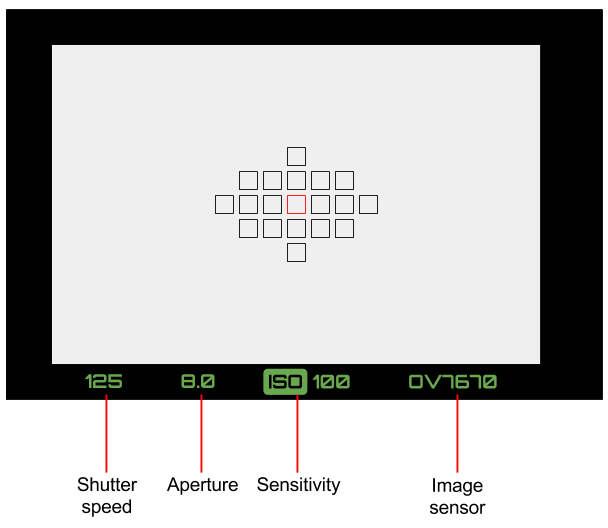
\includegraphics[width=1\textwidth]{./img/viewfinder.png}
  \caption{Mockup showing how the currently-installed sensor can be projected onto the viewfinder.}
  \label{fig:viewfinder}
\end{figure}

\subsection{Vendor extensions}
\gls{edid} also allows for vendor-specific extension blocks to be used which can be utilised here to add additional sensor-specific functionality. In order to add colour back to the RAW image the \gls{cfa} pattern must be known ahead of time in order to de-mosaic the image. While most image sensors implement the standard Bayer pattern, some image sensors, such as the Fuji X-Trans line, opt for exotic patterns which supposedly boast higher image quality. De-mosaicing an image with an incorrect \gls{cfa} pattern will result in unrealistic colour rendering, so it is essential that any part of the system which needs to perform de-mosaicing has an understanding of the \gls{cfa} pattern used on the image sensor. The most basic \gls{cfa} pattern is actually a 2 x 2 tiled array, so rather than storing the entire \gls{cfa} in the \gls{edid}, only the repeated tile needs to be stored.
%\section{Shutter synchronisation subsystem}
\section{Flash storage manager}

\begin{figure}
  \centering
  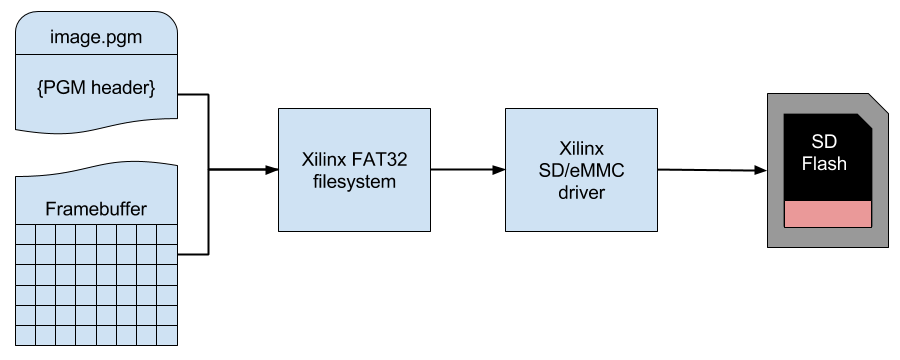
\includegraphics[width=1\textwidth]{./img/flash_storage.png}
  \caption{Framebuffer data is converted into PGM format and written to an SD card using Xilinx's FAT library.}
  \label{fig:flash_storage}
\end{figure}

Due to space constraints the framebuffer is only able to store a single frame at a time; upon receiving a new frame the previous frame is completely overwritten. Even if multiple frame buffers were used, the \SI{512}{\mega\byte} of DDR3 RAM inside the \gls{ps} would be filled after a few seconds of video. Instead, a flash-based SD card is used to store captured images when the shutter release is pressed. 

The Zybo development board used for this proof-of-concept system includes a multitude of built-in peripherals which can be accessed from both the \gls{pl} and the \gls{ps}. A MicroSD slot, SDIO 0, is provided as part of these peripherals and is connected to the \gls{ps} via multiplexed IO bank 1, lines 40--47. SD cards are typically able to run in two modes: SDIO mode (using the SDIO interface for high-throughput) and SPI mode (using the SPI interface for low-throughput). Higher throughput requires more resources and thus SPI mode is typically the preferred choice on resource-constrained microcontrollers. The ARM Cortex A9 inside the Zynq \gls{ps} is a fairly capable microprocessor however, and has full support for the SDIO interface via the SDIO peripheral controller. To read and write to the SD card the controller uses a 4-bit data interface with a maximum clock frequency of \SI{50}{\mega\hertz} for a theoretical transfer rate of \SI{25}{\mega\byte\per\second} --- of course this throughput is highly dependant on the type of data being transferred and the SD card used.

Writing to the SD card involves several layers of abstraction. The first abstraction layer is the Xilinx SD / eMMC library, which abstracts away the registers associated with operation of the SDIO peripheral controller which actually communicates with the SD card. One layer above that is Xilinx's FAT filesystem library which provides a very basic API for working with files stored in a FAT32 filesystem. FAT32 is supported on every major operating system, meaning that the SD card can be mounted and viewed on any system. It is also a relatively simple filesystem, making it the perfect choice for this proof-of-concept project which runs on bare-metal without the convenience provided by a full operating system such as embedded Linux. A Linux kernel for the Zynq platform was compiled from scratch as part of the project, however interfacing with any peripherals in the \gls{pl} would have required writing low-level kernel drivers which is far outside the scope of the project.

\begin{lstlisting}[caption={Using the Xilffs library to write the framebuffer to an SD card.}, label={lst:xilffs}, language=C]
FRESULT status;

// Mount the SD card to 0:/
status = f_mount(&fatfs, root_path, 0);
if (status != FR_OK) {
    return XST_FAILURE;
}

return XST_SUCCESS;

// Open a new PGM file for writing
status = f_open(&fh, filename, FA_CREATE_ALWAYS | FA_WRITE);
if (status != FR_OK) {
    return XST_FAILURE;
}

// Point the file pointer to the start of the file
status = f_lseek(&fh, 0);
if (status != FR_OK) {
    return XST_FAILURE;
}

(void)f_puts("P2\n640 480\n255\n", &fh);

// Flash data cache and write out pixel data
Xil_DCacheFlushRange((UINTPTR)g_framebuf, FRAMEBUF_WIDTH * FRAMEBUF_HEIGHT);
for (line=0; line<FRAMEBUF_HEIGHT; line++) {
    for (pixel=0; pixel<FRAMEBUF_WIDTH; pixel++) {
        f_printf(&fh, "%d ", g_framebuf[line][pixel]);
    }
    f_putc('\n', &fh);
}
\end{lstlisting}

Listing \ref{lst:xilffs} shows the Xilinx FAT filesystem library being used to write a frame to the SD card. Before the SD card can be used it must first be mounted using the \texttt{f\_mount()} function so the filesystem can be accessed --- this is immediately reminiscent of UNIX systems. Once the filesystem is mounted, the Xilffs library provides functions for file access, directory access, file / directory management and volume management \cite{xilinx:ug643}. To write a frame to the SD card the \texttt{f\_open()} function is called to open a file, specifying the \texttt{FA\_WRITE} flag to indicate the file is to be written to. Before any data can be written the file pointer must be positioned at the start of the file using the \texttt{f\_lseek()} function with an offset of zero. As with the framebuffer \gls{dma} processor, the data cache needs to be flushed before writing any data otherwise stale data will be used for the \gls{dma} transfer to the SD card. The Xilffs library supports multiple ways of writing to a file; the \texttt{f\_printf()} function is used here to write each pixel in the framebuffer to the file as integers delimited by spaces. It is important to finish any set of writes with a call to \texttt{f\_close()} to ensure that all bytes are committed to the disk.

Due to the transfer rates it is not possible to capture video using this method --- only still images can be captured. When doing anything requiring working with filesystems and high throughput it is generally desirable to use a full operating system with optimised filesystem code. While very lean, programming on bare-metal means not having many of the underlying mechanisms such as IO buffers, which are used to accelerate filesystem access to attain high throughput rates. The Xilinx FAT filesystem library is provided mainly for convenience --- to be able to log small quantities of data to an external SD card, not for pushing out 1080p video.

Because the entire framebuffer is written in one go, the framebuffer \gls{dma} processor is blocked from running. While the \glspl{isr} are still called, the framebuffer \gls{dma} transfers are initiated in the main process which is blocked by the SD card write. As the framebuffer \gls{dma} processor is inactive during this period the output linebuffer becomes stale, with the viewfinder controller rendering the same line repeatedly, causing the pixel smearing in Figure \ref{fig:interrupt_smudge}. While very simple, writing the entire frame in a single chunk is sub-optimal and several markedly better alternatives exist. Firstly, the ARM Cortex A9 inside the \gls{ps} is dual core, however the firmware is only single-threaded. Rather than running everything on a single core, it would be desirable to run critical tasks  (anything involving reading or writing to the framebuffer) on one core and non-critical code (rendering the viewfinder HUD) on the other. Another improvement would be the addition of a state machine; rather than writing the whole chunk in one go, a state machine could be used to break the SD card write into smaller chunks so that the framebuffer \gls{dma} processor can run in between.

\begin{figure}
  \centering
  
\includegraphics[width=0.5\textwidth]{./img/interrupt_smudge.jpg}
  \caption[Video output smudge due to blocking.]{Writing to flash storage prevents the framebuffer \gls{dma} processor from running, causing a smudged appearance as the same line is drawn repeatedly.}
  \label{fig:interrupt_smudge}
\end{figure}

\subsection{PGM image format}
Images are saved in \gls{pgm} ASCII format for convenient viewing on computers. \gls{pgm} is very basic greyscale image format designed to be platform-agnostic and thus fully portable between different systems. Typically a RAW format such as Adobe DNG would be used for storing RAW images as they are able to embed additional metadata such as the \gls{cfa} pattern and camera settings (aperture, focal length etc.) used. As a middle-ground between a completely proprietary binary format and standardised but complex RAW format, \gls{pgm} was chosen for its portability and simplicity.

When used in ASCII mode, \gls{pgm} data is encoded as ASCII data using space delimiters, rather than as binary values at specific offsets. The header is simply the magic string \texttt{P2} to identify the ASCII \gls{pgm} file format, followed by the width and height of the image in pixels, followed by \texttt{255}, the maximum value per pixel. The \gls{pgm} header used for the OV7670 image sensor is shown in Listing \ref{lst:pgm_header}.

\begin{lstlisting}[caption={\gls{pgm} file header.}, label={lst:pgm_header}]
P2          # P1 = Bitmap, P2 = Greymap, P3 = Pixmap
640 480     # OV7670 images are 640 x 480
255         # 8-bit pixel-depth
\end{lstlisting}

After the header the pixel data is written out as 480 lines of 640 ASCII-formatted integer values, with each value corresponding to a single pixel. As in the header, values are delimited by spaces. The resulting images are able to be viewed in any \gls{pgm} viewer, or converted to a more common filetype such as a Bitmap or PNG.
%\section{Viewscreen controller}
%\section{Test pattern generator}
%\section{Sequence detector}